\documentclass[landscape]{article}
\usepackage[landscape,margin=0.7in]{geometry}
\usepackage{pgfplots}
\usepackage{tikz}
\pgfplotsset{compat=1.18}

\begin{document}
\pagestyle{empty}

\begin{figure}
    \centering
    \begin{tikzpicture}
        \begin{axis}[
            title={\huge Comparison of Aircraft Boarding Strategies},
            ylabel={Remaining Passengers},
            xlabel={Time (minutes)},
            xmin=0,
            xmax=24,
            ymin=0,
            ymax=120,
            width=0.9\textwidth,
            height=0.5\textheight,
            legend style={at={(0.98,0.98)}, anchor=north east},
            grid=both
        ]
            % Random boarding curve
            \addplot[red, ultra thick] coordinates {
                (0, 114)
                (5, 85)
                (11, 57)
                (16, 29)
                (22, 0)
            };
            
            % Back-to-front boarding curve
            \addplot[blue, ultra thick] coordinates {
                (0, 114)
                (4, 76)
                (8, 38)
                (12, 0)
            };
            
            % Outside-in boarding curve
            \addplot[green, ultra thick] coordinates {
                (0, 114)
                (4, 76)
                (8, 38)
                (10, 0)
            };
            
            % Hybrid strategy boarding curve
            \addplot[purple, ultra thick] coordinates {
                (0, 114)
                (3, 89)
                (6, 62)
                (8, 35)
                (10, 0)
            };
            
            \legend{Random (22 min), Back-to-Front (12 min), Outside-In (10 min), Hybrid (10 min)}
        \end{axis}
    \end{tikzpicture}
\end{figure}

\begin{figure}
    \centering
    \begin{tikzpicture}
        \begin{axis}[
            title={\Large Comparison of Aircraft Boarding Strategies - Visualized Pattern},
            hide axis,
            scale only axis,
            width=0.8\textwidth,
            height=0.3\textheight
        ]
            % Just a placeholder to set up the diagram space
            \addplot coordinates {(0,0) (1,1)};
        \end{axis}
        
        % Now draw the boarding patterns manually
        
        % Random strategy
        \node[align=center] at (-5, 2) {\Large Random\\Strategy};
        \draw[rounded corners, fill=gray!20] (-8, 0) rectangle (-2, 1);
        \foreach \x in {-7.5, -7, -6.5, -6, -5.5, -5, -4.5, -4, -3.5, -3, -2.5}
            \foreach \y in {0.25, 0.5, 0.75}
                \filldraw[fill=purple!50, draw=black] (\x, \y) circle (0.1);
        
        % Back-to-front strategy
        \node[align=center] at (0, 2) {\Large Back-to-Front\\Strategy};
        \draw[rounded corners, fill=gray!20] (-3, 0) rectangle (3, 1);
        \draw[black, dashed] (-1, 0) -- (-1, 1);
        \draw[black, dashed] (1, 0) -- (1, 1);
        \node at (-2, 1.3) {Back};
        \node at (0, 1.3) {Middle};
        \node at (2, 1.3) {Front};
        
        \foreach \x in {-2.5, -2, -1.5}
            \foreach \y in {0.25, 0.5, 0.75}
                \filldraw[fill=blue!50, draw=black] (\x, \y) circle (0.1);
        \foreach \x in {-0.5, 0, 0.5}
            \foreach \y in {0.25, 0.5, 0.75}
                \filldraw[fill=blue!30, draw=black] (\x, \y) circle (0.1);
        \foreach \x in {1.5, 2, 2.5}
            \foreach \y in {0.25, 0.5, 0.75}
                \filldraw[fill=blue!10, draw=black] (\x, \y) circle (0.1);
        
        % Outside-in strategy
        \node[align=center] at (5, 2) {\Large Outside-In\\Strategy};
        \draw[rounded corners, fill=gray!20] (2, 0) rectangle (8, 1);
        \foreach \x in {2.5, 3, 3.5, 4, 4.5, 5, 5.5, 6, 6.5, 7, 7.5}
            \filldraw[fill=green!50, draw=black] (\x, 0.75) circle (0.1);
        \foreach \x in {2.5, 3, 3.5, 4, 4.5, 5, 5.5, 6, 6.5, 7, 7.5}
            \filldraw[fill=green!30, draw=black] (\x, 0.5) circle (0.1);
        \foreach \x in {2.5, 3, 3.5, 4, 4.5, 5, 5.5, 6, 6.5, 7, 7.5}
            \filldraw[fill=green!10, draw=black] (\x, 0.25) circle (0.1);
            
        % Legend
        \node[draw, align=left, anchor=south] at (0, -1) {
            \textbf{Summary of Boarding Strategies:}\\
            Random: No specific order, high passenger interference, longest time (22 min)\\
            Back-to-Front: Back zone first, then middle, then front (12 min)\\
            Outside-In: Window seats first, then middle seats, then aisle seats (10 min)\\
            Hybrid: Combines window-to-aisle and back-to-front principles (10 min)
        };
    \end{tikzpicture}
\end{figure}

\end{document}